\documentclass{beamer}
\usepackage[utf8]{inputenc}
\usepackage{verbatim}
\usepackage{minted}
\usepackage[spanish]{babel}
\usetheme{Frankfurt}
\usecolortheme{seahorse}
\useoutertheme{shadow}
\useinnertheme{circles}
\graphicspath{ {./figures/} }
\title[Laboratorio]{Herramientas de trabajo}
\author[Miguel]{Miguel Angel Piña Avelino}
\institute[UNAM]{
  Ingeniería de Software,\\
  Facultad de Ciencias, UNAM
}
\AtBeginSection[]{
  \begin{frame}
  \vfill
  \centering
  \begin{beamercolorbox}[sep=8pt,center,shadow=true,rounded=true]{title}
    \usebeamerfont{title}\insertsectionhead\par%
  \end{beamercolorbox}
  \vfill
  \end{frame}
}


\date{\today}
\begin{document}

\frame{\titlepage}
\begin{frame}
  \frametitle{Índice}
  \tableofcontents
\end{frame}

\section{¿Qué es Maven?}

\begin{frame}
  \frametitle{¿Qué es Maven?}
  \begin{itemize}[<+->]
  \item Herramienta para la gestión y construcción de proyectos en Java.
  \item Tiene un funcionamiento similar al de Ant.
  \item Trabaja sobre configuraciones en xml.
  \item Proyecto de nivel superior de la Apache Software Fundation.
  \item Utiliza Project Object Models (POM) para describir el proyecto a construir.
  \item Esta listo para usarse desde la red.
  \end{itemize}
\end{frame}

\section{Filosofía de Maven}

\begin{frame}
  \frametitle{Filosofía de Maven}
  \begin{itemize}[<+->]
  \item Estandarización de las construcciones.
  \item Convención sobre configuración.
  \item Restringe ampliamente la variabilidad de construir proyectos de software.
  \item Es ideal para proyectos nuevos.
  \item Los proyectos complejos y existentes podrían no ser adaptables a Maven.
  \end{itemize}
\end{frame}

\section{¿Cómo funciona Maven?}

\begin{frame}[fragile]
  \frametitle{¿Cómo funciona Maven?}
  \begin{figure}[ht]
    \centering
    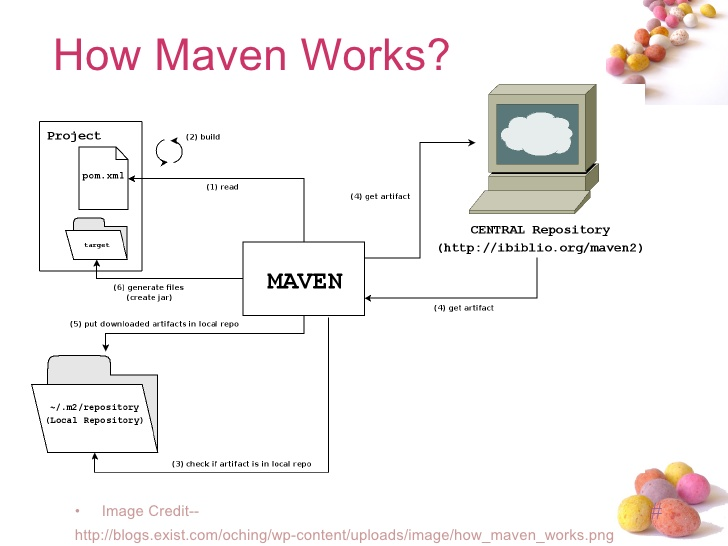
\includegraphics[scale=0.4]{figures/how-maven-works.jpg}
    \caption{\label{fig:maven} ¿Cómo funciona Maven?}
  \end{figure}

\end{frame}

\begin{frame}
  \frametitle{Ciclo de vida}
  \begin{itemize}[<+->]
    \item \textbf{Compile}: Genera archivos .class desde los fuentes .java
    \item \textbf{Test}: Ejecuta las pruebas automáticas de JUnit existentes, abortando el
          proceso de ejecución de maven si alguno de estos fallan.
    \item \textbf{Package}: Genera archivos .jar ó .war con los .class compilados.
    \item \textbf{Install}: Copia el fichero .jar (.war) a una carpeta donde Maven comparte
          todos los .jar generados. Esto permite que un mismo proyecto esté
          disponible para otros.
    \item \textbf{Deploy}: Copia el .jar a un servidor remoto, poniéndolo disponible para
          cualquier proyecto maven con acceso a un servidor remoto.

   \end{itemize}

 \end{frame}

 \begin{frame}
   \frametitle{Ciclo de vida}
   Cuando se ejecuta alguno de los comandos anteriores, por ejemplo,
   mvn install, maven irá verificando que todas las faces previas a el se
   hayan cumplido.
 \end{frame}

 \begin{frame}
   \frametitle{Metas adicionales}

   Maven también tiene disponibles algunas metas que están fuera del ciclo de vida
   que pueden ser llamadas, pero Maven asume que estas metas no son parte del ciclo
   de vida estándar.

 \end{frame}

 \begin{frame}
   \frametitle{Metas adicionales}
   \begin{itemize}[<+->]
   \item \textbf{Clean}: Elimina todos los \textsl{.class} y \textsl{.jar} generados.
   \item \textbf{Assembly}: Genera un archivo \textsl{.zip} con todo lo necesario para instalar
     nuestro programa java. Se debe configurar previamente en un fichero \textsl{.xml}
     que se debe incluir en ese zip.
   \item \textbf{Site}: Genera un sitio web con la información de nuestro proyecto.
   \item \textbf{Site-deploy}: Sube el sitio web anterior.
   \end{itemize}
 \end{frame}

\section{Creando un primer proyecto en Maven}

\begin{frame}[fragile]
   \frametitle{Creando un primer proyecto en Maven}
   Para crear un proyecto Maven simple, basta con ejecutar la
   siguiente instrucción (previamente con maven instalado).

   \begin{minted}{sh}
     mvn archetype:generate\
     -DgroupId="com.miguel.proyecto"\
     -DartifactId="mi-proyecto" -Dversion="0.0.1"
   \end{minted}
\end{frame}

\begin{frame}
  \frametitle{Creando un primer proyecto en Maven}
     El código anterior va a crear un proyecto de maven con una serie de paquetes por
     defecto para diferenciarlo de otros proyectos \texttt{com.miguel.poyecto}, así como tener
     por nombre \texttt{mi-proyecto} y empezar con la versión \texttt{0.0.1}.
\end{frame}

\begin{frame}[fragile]
  \frametitle{Creando un primer proyecto en Maven}

  \begin{figure}[ht]
    \centering
    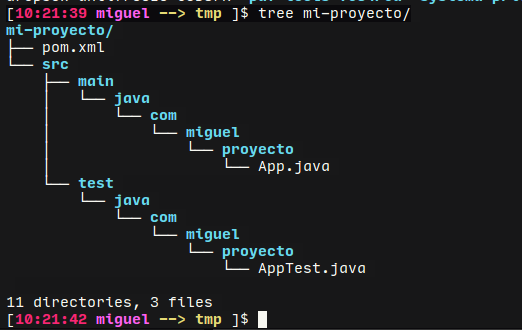
\includegraphics[scale=0.5]{figures/mvn1.png}
    \caption{\label{fig:maven1} Estructura de un proyecto de Maven}
  \end{figure}

\end{frame}

\begin{frame}
  \frametitle{Creando un primer proyecto en Maven}
  Podemos editarlo, compilarlo y jugar un poco con el proyecto.

  Para que pueda agregar la referencia de donde se encuentra el archivo principal
  (main) dentro del jar, esto una vez que sea empaquetado, hay que agregar la
  siguiente instrucción en el pom.xml, justo después de las dependencias del
  proyecto
\end{frame}

\begin{frame}[fragile]
  \frametitle{Creando un primer proyecto en Maven}

  \begin{minted}[fontsize=\scriptsize]{xml}
<build>
  <plugins>
	<plugin>
	  <groupId>org.apache.maven.plugins</groupId>
	  <artifactId>maven-jar-plugin</artifactId>
	  <configuration>
		<archive>
		  <manifest>
			<mainClass>com.miguel.proyecto.App</mainClass>
		  </manifest>
		</archive>
	  </configuration>
	</plugin>
  </plugins>
</build>
\end{minted}

Estableciendo el archivo main dentro del proyecto.

  % \begin{figure}[ht]
  %   \centering
  %   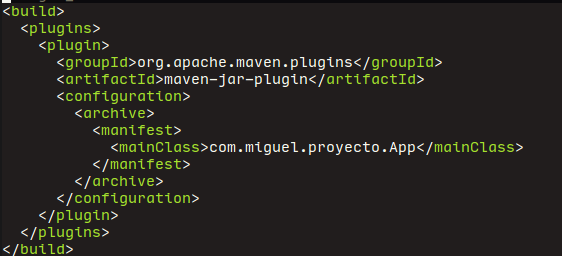
\includegraphics[scale=0.5]{figures/mvn2.png}
  %   \caption{\label{fig:maven2} Indicando cual es el archivo Main}
  % \end{figure}

\end{frame}

\section{Creando un proyecto web con Maven}

\begin{frame}[fragile]
  \frametitle{Creando un proyecto web con Maven}
  De forma similar al ejemplo anterior, para construir un proyecto, podemos hacer
  uso de las herramientas que maven nos provee para construir una
  aplicación web.

  \begin{minted}{sh}
    mvn archetype:generate \
    -DgroupId="com.miguel.proyecto" \
    -DartifactId="mi-primer-aplicacion-web" \
    -DarchetypeArtifactId=maven-archetype-webapp \
    -DinteractiveMode=false
  \end{minted}
\end{frame}

\begin{frame}[fragile]
  \frametitle{Creando un proyecto web con Maven}
  \begin{figure}[ht]
    \centering
    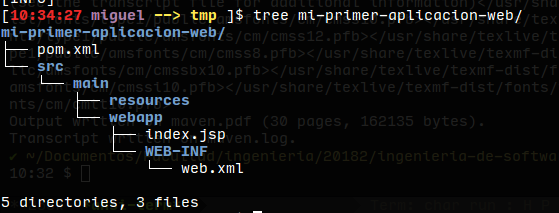
\includegraphics[scale=0.5]{figures/mvn3.png}
    \caption{\label{fig:maven3} Estructura de un proyecto web}
  \end{figure}

\end{frame}

\begin{frame}[fragile]
  \frametitle{Incluyendo un servidor HTTP}
  Para tener un servidor http integrado con la aplicación, basta con agregar el
  siguiente snippet al archivo pom.xml

  \begin{minted}[fontsize=\tiny]{xml}
<build>
  <finalName>mi-primer-aplicacion-web</finalName>
  <plugins>
	<!-- Set JDK Compiler Level -->
	<plugin>
	  <groupId>org.apache.maven.plugins</groupId>
	  <artifactId>maven-compiler-plugin</artifactId>
	  <version>2.3.2</version>
	  <configuration>
		<source>${jdk-version}</source>
		<target>${jdk-version}</target>
	  </configuration>
	</plugin>

	<!-- For Maven Tomcat Plugin -->
	<plugin>
	  <groupId>org.apache.tomcat.maven</groupId>
	  <artifactId>tomcat7-maven-plugin</artifactId>
	  <version>2.2</version>
	  <configuration>
		<path>/mi-primer-aplicacion-web</path>
	  </configuration>
	</plugin>

  </plugins>
</build>
  \end{minted}

  % \begin{figure}[ht]
  %   \centering
  %   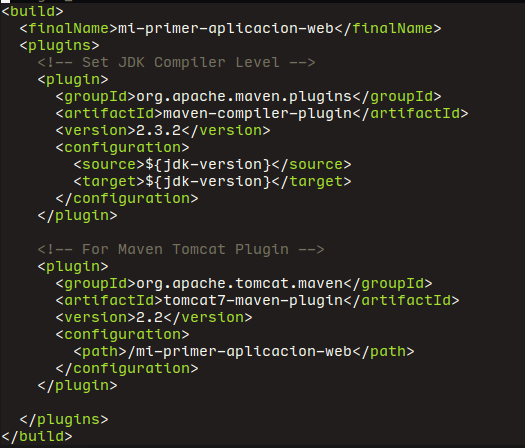
\includegraphics[scale=0.37]{figures/mvn4.png}
  %   \caption{\label{fig:maven4} Incluyendo un servidor HTTP}
  % \end{figure}
\end{frame}

\begin{frame}[fragile]
  \frametitle{Incluyendo un servidor HTTP}
  Para ejecutarlo, primero hay que construir el proyecto

\begin{minted}[fontsize=\small]{sh}
mvn clean install
\end{minted}

y después verificar que funciona

\begin{minted}[fontsize=\small]{sh}
mvn tomcat:run
\end{minted}

En un navegador web entramos a la url

\begin{minted}[fontsize=\small]{sh}
http://localhost:8080/mi-primer-aplicacion-web/
\end{minted}

\end{frame}

\begin{frame}
  \frametitle{Estructura del proyecto}
  A diferencia del primer proyecto maven con el que trabajamos, en este vamos a
  tener un archivo especial: \textbf{web.xml}.

  Este archivo es conocido \texttt{Deployment Descriptor} que es utilizado para determinar
  como las URL van a ser \texttt{mapeadas} a Servlets de java.
\end{frame}

\begin{frame}
  \frametitle{Estructura del proyecto}
  Va a describir las clases, recursos y la configuración de la aplicación y cómo
  el servidor web va utilizar la información anterior para resolver peticiones
  web. Cuando un servidor web recibe una petición para la aplicación, se usa el
  \texttt{deployment descriptor}  para mapear la URL de la petición al código que puede
  responder a dicha petición.
\end{frame}

\begin{frame}
  \frametitle{Agregando servlets al proyecto}
  Un servlet, es una clase de Java que es utilizada para responder a las
  solicitudes http que llegan a un servidor. Estos servlets van a extender a la
  clase abstracta HttpServlet y van a sobreescribir al menos dos de los métodos
  utilizados para responder peticiones web: \textbf{doGet} y \textbf{doPost}.
\end{frame}

\begin{frame}[fragile]
  \frametitle{Agregando servlets al proyecto}
  Los servlets son definidos en el \textbf{deployment descriptor}, como se ejemplifica a
  continuación:

  \begin{minted}[fontsize=\scriptsize]{xml}
<!DOCTYPE web-app PUBLIC
 "-//Sun Microsystems, Inc.//DTD Web Application 2.3//EN"
 "http://java.sun.com/dtd/web-app_2_3.dtd" >

<web-app>
  <display-name>Archetype Created Web Application</display-name>
      <servlet>
        <servlet-name>servlet</servlet-name>
        <servlet-class>com.miguel.proyecto.Servlet</servlet-class>
    </servlet>
    <servlet-mapping>
        <servlet-name>servlet</servlet-name>
        <url-pattern>/foo</url-pattern>
    </servlet-mapping>
</web-app>
  \end{minted}
\end{frame}


\begin{frame}[fragile]
  \frametitle{Agregando un servlet al proyecto}
  En este descriptor agregamos un servlet llamado \textbf{servlet}, que tiene asociada a la
  clase \texttt{com.miguel.proyecto.Servlet}. Esta clase va a responder a las peticiones
  que lleguen a la url \textbf{/mi-proyecto/foo}, el servlet de ejemplo es el siguiente:
\end{frame}

\begin{frame}[fragile]
  \frametitle{Agregando un servlet al proyecto}
  \begin{minted}[fontsize=\scriptsize]{java}
  package com.miguel.proyecto;

  import java.io.IOException;
  import java.io.PrintWriter;
  import javax.servlet.ServletException;
  import javax.servlet.http.HttpServlet;
  import javax.servlet.http.HttpServletRequest;
  import javax.servlet.http.HttpServletResponse;

  @SuppressWarnings("serial")
  public class Servlet extends HttpServlet {

      private void foo(HttpServletRequest request, HttpServletResponse
      response) throws ServletException, IOException {
          response.setContentType("text/html");
          PrintWriter pw = response.getWriter();
          pw.println("<HTML><HEAD><TITLE>Leyendo parámetros</TITLE></HEAD>");
          pw.println("<BODY BGCOLOR=\"#CCBBAA\">");
          pw.println("<H2>Leyendo parámetros desde un formulario html</H2><P>");
          pw.println("<UL>\n");
          pw.println("</BODY></HTML>");
          pw.close();
      }
  \end{minted}

\end{frame}

\begin{frame}[fragile]
  \frametitle{Agregando un servlet al proyecto}
  \begin{minted}[fontsize=\scriptsize]{java}
      @Override
      protected void doGet(HttpServletRequest request,
      HttpServletResponse response) throws ServletException,
      IOException {
          foo(request, response);
      }

      @Override
      protected void doPost(HttpServletRequest request,
      HttpServletResponse response) throws ServletException
      IOException {
          foo(request, response);
      }
  }
  \end{minted}
\end{frame}

\begin{frame}[fragile]
  \frametitle{Agregando servlets al proyecto}
  para que la clase anterior funcione, hay que agregar el siguiente snippet de
código al archivo pom.xml

\begin{minted}[fontsize=\scriptsize]{xml}
  <dependency>
    <groupId>javax.servlet</groupId>
    <artifactId>javax.servlet-api</artifactId>
    <version>3.1.0</version>
    <scope>provided</scope>
  </dependency>
\end{minted}

\end{frame}

\begin{frame}[fragile]
  \frametitle{Agregando un servlet al proyecto}
  Lo anterior va a agregar todas las dependencias necesarias para poder construir
  de nueva cuenta nuestro proyecto:

\begin{minted}[fontsize=\small]{sh}
mvn clean install
mvn tomcat:run
\end{minted}

Y entramos a la url

\begin{minted}[fontsize=\small]{sh}
http://localhost:8080/mi-primer-aplicacion-web/foo
\end{minted}

\end{frame}

\end{document}
